\clearpage
\maketitlesupplementary
\appendix

In this Supplement, we provide additional implementation details in \cref{sec:impl}, a discussion of common data issues in \cref{sec:data_quality}, and a discussion of limitations in \cref{sec:limitation}.

\section{Additional Details}%
\label{sec:impl}

In this section, we detail the training setup and architecture (\cref{sec:impl-training}), the construction of positive and negative pairs (\cref{sec:impl-pairs}), the VLM prompt (\cref{sec:impl-vlm-prompt}), the annotation filtering criteria (\cref{sec:impl-filtering}), and the language alignment procedure (\cref{sec:impl-language-alignment}).

\subsection{Training and Architecture}%
\label{sec:impl-training}

To train our model, we set the loss weights in \cref{eq:training-loss} to $\lambda_{\text{cam}} = 5.0$, $\lambda_{\text{depth}} = 1.0$, $\lambda_{\text{point}} = 0.5$, and $\lambda_{\text{match}} = 0.1$.
For each scene, following~\cite{wang24dust3r:, wang25vggt}, we normalize the ground truth to a unit space.
Concretely, we first transform all quantities into the first camera's coordinate frame and compute the average distance of all 3D points to the origin; we then scale the depth maps and translation vectors by this value.
As in~\cite{wang25vggt}, this normalization is applied only to the ground truth and not to the predictions.
To stabilize training, we apply gradient-norm clipping with a threshold of $1.0$ and use QKNorm inside the attention layers.
At each iteration, we randomly sample the number of input frames from the range $[1, 24]$ and correspondingly set the batch size to saturate GPU memory.
Each frame is independently masked by a rectangle whose height and width are uniformly sampled from $[32, 128]$ pixels, with a probability of $0.05$.
Pixels inside the masked region are set to black, and the corresponding depth values are marked as invalid.
For color jittering, we use PyTorch's implementation with brightness $0.5$, contrast $0.5$, saturation $0.5$, and hue $0.1$.
During self-supervised training, the weights of the teacher model are updated using an exponential moving average with a decay of $0.999$.
Our camera head follows the implementation in~\cite{wang25vggt}, using a ReLU activation for the focal length and no activation for the quaternion and translation parameters.
For datasets with temporally ordered sequences (\eg, videos), we sample frames from a local temporal window rather than based on covisibility.
This can produce particularly challenging reconstruction subsets in which images are semantically related but share little or no visual overlap.
We found that these samples improve the model's generalization.

\subsection{Constructing Positive and Negative Pairs}%
\label{sec:impl-pairs}

We expand on the matching loss introduced in the main paper (\cref{sec:training-losses}) by detailing how we construct the positive and negative token pairs.

Given per-pixel 3D points obtained by unprojecting the depth maps, we first sample valid pixels in the query frame and assign each sampled pixel to a query patch.
Using the known camera intrinsics and extrinsics, we then project the corresponding 3D points into all other frames and retain only those projections that (i) fall inside the image and (ii) are depth-consistent with the target-frame depth maps (within a small relative tolerance of $1\%$ and excluding a narrow image boundary of 4 pixels).

For each target frame, we count how many 3D points from each query patch land in each target patch.
This yields, for every query patch, a soft correspondence map over target patches in the form of projection overlap ratios.
We select query patches that have sufficient valid projections across views and randomly sample up to a fixed number of them, with sampling probabilities proportional to their total number of correspondences.
For each selected query patch, all target patches with $>$10\% overlap form positive token pairs.

Because some sequences are dynamic, failing the positive-pair criteria does not automatically define a valid negative.
Instead, we construct negative pairs by randomly sampling patches as query and target candidates, and then enforcing two constraints:
(i) a geometric constraint, requiring the candidate target patch center to lie sufficiently far from the epipolar line induced by the query patch (\ie, to have a large epipolar/Sampson distance), and
(ii) an appearance constraint, requiring a sufficiently large \(\ell_2\) distance between the mean RGB values of the two patches.
Patches that satisfy both constraints are treated as negatives.
We then subsample these negatives to obtain a balanced set of positive and negative patch pairs for supervising the matching loss on the last-layer tokens.

\subsection{VLM Prompt}%
\label{sec:impl-vlm-prompt}

We use a VLM to discard videos not suitable for multi-view geometry.
We prompt the VLM as follows:

{
  \vspace{1em}
  \color{linegreen}
  \hrule
  \vspace{1pt}
  \hrule
  \vspace{0.5em}
}

\begingroup

\color{promptcolor} \ttfamily \footnotesize \raggedright
\noindent
"You are an expert in computer vision, photogrammetry, and Multi-View Geometry (MVG)."\\
"Analyze the video clip to determine if it is suitable for high-quality 3D reconstruction."\\
"You must categorize the video and extract scene metadata based on the strict criteria below."

\vspace{0.5em}
\noindent {STEP 1: CHECK FOR HARD REJECTION FACTORS} \\
``Assess the following. If ANY are present, the Classification is {`REJECT\_HARD'}'':
\begin{enumerate}[noitemsep, topsep=0pt, leftmargin=*]
    \item Discontinuities \& Editing: Does the video contain cuts, dissolves, wipes, fades, or montage editing? (Must be a single continuous shot).
    \item Non-Physical/2D Content: Is this a screen recording, a slideshow of static images, animation, or a cartoon? (Must be real-world footage).
    \item Extreme Visual Failure: Severe motion blur (edges lost), severe rolling shutter (wobble/jello effect), or corruption/glitching.
    \item Major Obstructions: Are there heavy overlays (large text/UI), watermarks, or physical obstructions like a finger covering the lens?
    \item Non-Pinhole Projections: Is the footage 360$^{\circ}$ equirectangular or heavily distorted fisheye without calibration?
\end{enumerate}

\vspace{0.5em}
\noindent {STEP 2: CHECK FOR GEOMETRIC \& TEXTURAL SUITABILITY} \\
"If the video passes Step 1, assess for reconstruction quality. If ANY are present, the Classification is {`REJECT\_SOFT'}:"
\begin{enumerate}[noitemsep, topsep=0pt, leftmargin=*]
    \item Insufficient Parallax: Is the camera stationary? Does it only rotate (pan/tilt) or zoom without physical translation? (Translation is required for depth).
    \item Texture Issues: Does the scene lack non-repetitive texture? (e.g., blank white walls, clear blue sky only, dark shadows, or highly repetitive patterns like grid tiles).
    \item Specularities \& Transparencies: Are the dominant features reflective (mirrors, water, glass) or transparent? (These create `ghost' geometry).
    \item Focus \& DOF Issues: Is there severe focus hunting (pulsing), or is the depth-of-field so shallow that the background is entirely blurred (bokeh)?
    \item Dynamic Dominance: Is the frame dominated ($>$90$\%$) by a moving subject (e.g., a close-up talking head) while the static background is visible but minimal?
\end{enumerate}

\vspace{0.5em}
\noindent {STEP 3: EXTRACT METADATA}\\
"Determine the scene dynamics:"
\begin{enumerate}[noitemsep, topsep=0pt, leftmargin=*]
    \item Dynamic: Moving objects are present (people walking, cars moving, wind blowing trees heavily).
    \item Static: The scene is rigid; only the camera is moving.
\end{enumerate}

\vspace{0.5em}
\noindent {OUTPUT INSTRUCTIONS:} \\
"Return a JSON object strictly following this schema. Do not output markdown formatting or explanations outside the JSON."
\begin{verbatim}
{
"classification": 
"ACCEPT" | "REJECT_HARD" | "REJECT_SOFT",
"reason": "Brief descriptions of the primary 
flaw or 'Good candidate'",
"scene_dynamics": "Static" | "Dynamic"
}
\end{verbatim}

\noindent "Label Definitions:" \\
{REJECT\_HARD}: Unusable due to editing, synthetic content, severe artifacts, or obstructions. \\
{REJECT\_SOFT}: Technically usable but risks failure due to rotation-only, reflections, lack of texture, or focus issues. \\
{ACCEPT}: High-quality candidate. Single shot, clear translation/parallax, good texture, rigid geometry.
\endgroup

{
  \vspace{0.5em}
  \color{linegreen}
  \hrule
  \vspace{1pt}
  \hrule
  \vspace{1em}
}


\subsection{Annotation Filtering Criteria}%
\label{sec:impl-filtering}

To train the ensemble classifier (XGBoost, Random Forest, and CatBoost) described in \cref{sec:annotation-pipeline}, we extract several geometric features from each reconstruction.
These features are designed to detect common failure modes such as collinear motion degeneracies, inconsistent scale, and noisy camera trajectories.
Below, we provide definitions for the most important features implemented in our pipeline.

\paragraph{Trajectory Smoothness.}

We quantify the smoothness of the estimated camera trajectory using the acceleration of the translation vectors $\mathbf{t}$.
The smoothness score $S_\text{trans}$ is calculated as the mean squared magnitude of the acceleration:
\begin{equation}
    S_\text{trans} = \frac{1}{N-2} \sum_{i=1}^{N-2} \| \mathbf{t}_{i+1} - 2\mathbf{t}_i + \mathbf{t}_{i-1} \|^2
\end{equation}
We compute a similar metric $S_\text{rot}$ for rotations using the second order difference of the rotation vectors.
High values in $S_\text{trans}$ or $S_\text{rot}$ indicate jittery trajectories, often associated with poor SfM convergence.

\paragraph{Parallax Angle Analysis.}

To ensure sufficient baseline for multi-view stereo, we analyze the parallax angles of the reconstructed sparse point cloud.
For a subset of sparse points $\mathcal{P}$, we identify the set of cameras $\mathcal{C}_p$ visible to point $p \in \mathcal{P}$.
We compute the maximum angle subtended by any pair of cameras $c_j, c_k \in \mathcal{C}_p$ at point $p$.
The final feature is the {median} of these maximum angles across all sampled points.
Low median parallax indicates degenerate rotation-only motion or extreme distance.

\paragraph{Point Cloud PCA Shape (Linearity \& Planarity).}

To detect geometric degeneracies such as ``fly-by'' straight-line reconstructions (which result in cylindrical ambiguity), we perform Principal Component Analysis (PCA) on the normalized point cloud coordinates.
Let $v_1 \ge v_2 \ge v_3$ be the eigenvalues of the point cloud covariance matrix.
We define \emph{Linearity} as $(v_1 - v_2) / v_1$, \emph{Planarity} as $(v_2 - v_3) / v_1$, and \emph{Scattering} as $v_3 / v_1$.
Reconstructions with excessively high linearity are flagged as linear degeneracies and are typically discarded by the classifier.

\paragraph{Depth Map Completeness.}

This metric evaluates the density of the dense reconstruction stage.
For each frame, we calculate the percentage of pixels containing valid, finite depth values relative to the total image resolution.
The final feature is the average completeness across all frames.
Extremely low values typically indicate failure in the Multi-View Stereo stage, often caused by textureless surfaces, high specularities, or bad cameras.

\paragraph{Point Cloud Noise Level.}

We estimate the signal-to-noise ratio using statistical outlier detection.
For every point, we compute the average distance to its nearest neighbors.
Points are classified as noise if this distance exceeds the global average by more than two standard deviations.
The feature is the percentage of points classified as noise, which allows us to detect reconstructions plagued by floating artifacts and outliers.

Note that this pipeline can provide depth values only for rigid pixels, so the metrics above assume that dynamic pixels are already masked out.
We assume the model can learn to estimate depth for dynamic pixels from synthetic data.

\subsection{Language Alignment}%
\label{sec:impl-language-alignment}

In \cref{sec:applications}, we use a VLM to produce a sequence-level language embedding for each training sequence.
Here, we provide the exact VLM prompt and representative generated descriptions.
The hidden states of the generated text tokens are mean-pooled and projected to form the language embedding.
The prompt and image tokens are excluded from this pooling.
We use at most \(128\) newly generated tokens and keep the VLM fixed.
The \method side is optimized during alignment fine-tuning, as described in \cref{sec:applications}.
The images are provided as an unordered collection, both to the VLM and to our model.

{
  \vspace{1em}
  \color{linegreen}
  \hrule
  \vspace{1pt}
  \hrule
  \vspace{0.5em}
}

\begingroup

\color{promptcolor} \ttfamily \footnotesize \raggedright
\noindent {\normalfont\bfseries Language Alignment Prompt}

\vspace{0.25em}
\noindent
These images show the same scene from multiple viewpoints.\\
Describe the full scene as one coherent scene, not as separate images.\par\vspace{0.5em}\noindent
Use the following format:\\
Scene: \textless{}scene category or environment\textgreater{}.\\
Content: \textless{}main objects and coarse spatial arrangement\textgreater{}.\\
Appearance: \textless{}stable visual attributes such as material, color, or style\textgreater{}.\par\vspace{0.5em}\noindent
Write one short sentence for each field.\\
Mention information that is consistent across multiple views, even if it is not visible in every view.\\
Focus on shared scene content, major objects, coarse layout, and stable appearance.\\
Mention dynamic objects only if they are prominent and identifiable in multiple views.\\
Do not describe motion, actions, or frame-specific changes.\\
Do not describe each image separately.\\
Do not mention camera motion, viewpoint order, image quality, blur, exposure, lighting artifacts, or uncertainty.\\
Keep the description concise, factual, and semantically dense.

\vspace{0.7em}
{\color{linegreen}\hrule height 0.6pt}
\vspace{0.6em}
\noindent {\normalfont\bfseries Representative Descriptions}
\vspace{-0.6em}
\newcommand{\exampleDashedSep}{\par\vspace{0.4em}\noindent{\color{linegreen}\leaders\hbox{\rule{0.8em}{0.4pt}\hspace{0.35em}}\hfill\kern0pt}\par\vspace{0.4em}}

\exampleDashedSep
\noindent Scene: A dimly lit room with a red hue, featuring a door, a window, and a wall with a patterned texture.\\
Content: The room contains a closed door on the left, a window on the right, and a wall with a textured pattern.\\
Appearance: The walls have a floral or damask pattern, the floor is dark, and the overall lighting is red.

\exampleDashedSep
\noindent Scene: Snowy forest landscape with a winding road.\\
Content: A snow-covered forest with tall pine trees, a winding road, and a steep slope.\\
Appearance: The scene has a high-contrast look, with dark clouds above and bright white snow covering the ground and trees.

\exampleDashedSep
\noindent Scene: Outdoor public area.\\
Content: A dark green plastic picnic table with a hexagonal top and black legs, accompanied by matching benches, situated on a paved surface.\\
Appearance: The table and benches are made of uniform dark green plastic with a matte finish, and the ground is composed of light gray square tiles.

\exampleDashedSep
\noindent Scene: Urban plaza with modern architecture.\\
Content: A central fountain with a large circular sculpture, surrounded by paved walkways and buildings.\\
Appearance: The fountain has a metallic, silver-colored structure with a dark base, and the surrounding area features light gray stone tiles and modern buildings with glass and concrete facades.

\endgroup

{
  \vspace{0.5em}
  \color{linegreen}
  \hrule
  \vspace{1pt}
  \hrule
  \vspace{1em}
}

\section{Data Quality}%
\label{sec:data_quality}

One of the most important ingredients for training large `foundation' models is data.
Having access to a large amount of data is, however, insufficient; in fact, the \emph{quality} of the data also has a strong effect on the model's behavior.
For 3D reconstruction, we found that noisy data introduces particular failure modes in both self-supervised and supervised training.

For self-supervised training, we observe that unreasonably difficult videos, such as the ones containing discontinuous shot transitions as commonly seen in television footage, induce sharp loss spikes and may cause gradients to explode, resulting in a degradation of the model's performance.
We therefore restrict self-supervised training to videos that pass the VLM pre-filtering check of \cref{sec:annotation-pipeline}, which reliably removes such cases.

In the supervised stage, the effects of noisy data are more subtle but equally important.
We find that different types of errors in the annotations translate into specific failure modes at inference time.
What is worse, these failure modes do not affect most of the images in standard benchmarks and may thus not be detected in the quantitative results.
Instead, they emerge only when the model is tested on a new sample that resembles an incorrectly labeled sample seen during training.
This behavior indicates that, while the model does learn the general principles of 3D reconstruction, it can nevertheless memorize idiosyncratic noise as well.
Next, we discuss the most representative cases we have encountered.

\begin{figure}
\centering
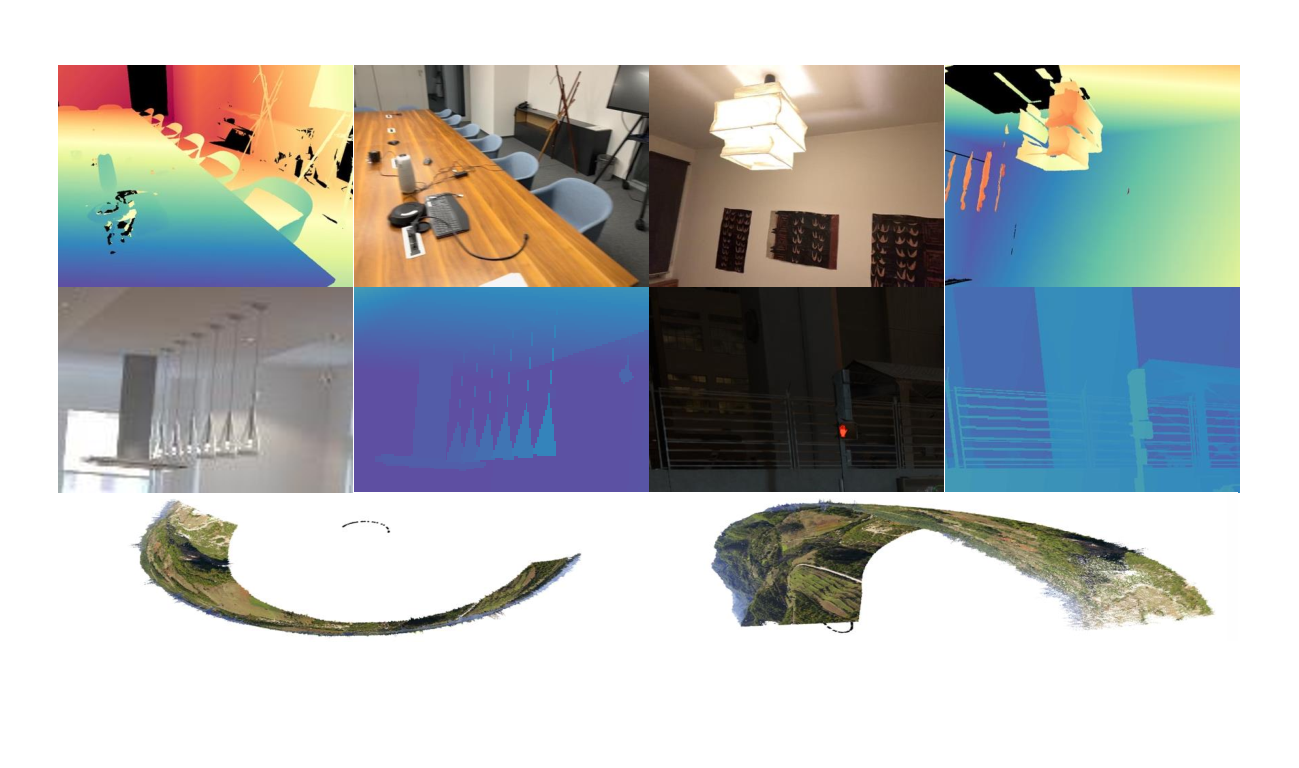
\includegraphics[width=0.95\linewidth]{figures/data_v3.pdf}
\caption{\textbf{Common Data Issues.}
Top: examples from ScanNet++.
Middle: examples from synthetic datasets such as Hypersim.
Bottom: the doming effect.}%
\label{fig:data_quality}
\vspace{-8pt}
\end{figure}




\paragraph{Sensors.}

Some datasets annotate real-world scenes using sensors such as LiDAR or depth cameras.
A common failure mode here is foreground-background leakage.
For example, as shown in the top row of~\cref{fig:data_quality} with an example from ScanNet++, the depth of the chair's back corresponds to the background floor or wall, likely due to misalignment or holes in the sensor capture.
We also observe spurious depth artifacts around the hanging light fixture, where the rendered depth contains fragmented foreground structures that do not correspond to the visible lamp geometry.
Such artifacts are likely caused by unreliable sensor capture or reconstruction around over-exposed and partially translucent objects.
We therefore exclude such datasets in the later phase of training.

\paragraph{Thin Structure.}

Synthetic data usually provides more accurate geometric annotations, but thin structures can be inaccurate in some synthetic datasets too.
Objects such as fence bars often occupy only a few pixels and lie on sharp depth discontinuities.
Although these structures are clearly visible in the RGB image, their rendered depth can be incomplete, overly smoothed, or misaligned.
As a result, the label may assign a thin structure to the depth of the wall, window, floor, or distant background behind it, rather than to the actual object surface, as shown in the middle row of~\cref{fig:data_quality}.
At inference time, the model may ignore thin objects, recover only their thicker or lower parts, or produce depth maps in which thin structures are washed out by nearby large surfaces.
This is a common problem in existing models, and we hypothesize that it can be mitigated with higher-resolution inputs or better synthetic data.

\paragraph{Fake Background.}

Another common issue in synthetic data is fake background.
For example, in Kubric, PointOdyssey, BEDLAM, the background depth may correspond to proxy dome or floor geometry used for HDRI rendering, rather than the true 3D structure suggested by the appearance of the background.
Although this is reasonable for rendering, it provides depth values that are inconsistent with the scene semantics.
For datasets with a clear boundary between the real foreground and the synthetic background, such as BEDLAM, we filter out the background during training by thresholding the maximum valid foreground depth.
We exclude the remaining from training.

\paragraph{Doming Effect.}

Methods using bundle adjustment, such as COLMAP~\cite{schonberger16structure-from-motion}, MegaSaM~\cite{li25megasam:}, and ViPE~\cite{huang25vipe:}, can be used to generate pseudo ground truth.
However, care is needed because they may produce degenerate solutions such as the doming effect, as shown in the bottom row of~\cref{fig:data_quality}.
This usually arises from weak global constraints in the image collection, \eg, near-parallel viewing directions, insufficient loop closure, small triangulation angles, or inaccurate camera self-calibration, especially radial-distortion errors, which are common in Internet videos.
Under these conditions, bundle adjustment can still achieve a low reprojection error while bending the recovered cameras and scene geometry into a globally inconsistent curved shape.
Such reconstructions may appear locally plausible but provide incorrect large-scale geometry, making them harmful as supervision.
They can be filtered out by supervised geometric filtering, as discussed in~\cref{sec:data}, or by comparing the annotated depths with predictions from existing monocular depth models or feed-forward reconstruction models.

\paragraph{Humans in Walls.}

We observe a recurring failure case in near-static street-view videos with pedestrians moving through the scene: almost all existing feed-forward reconstruction models often absorb humans into the static background, estimating them as part of nearby walls or buildings.
This failure appears to be related to ambiguous boundary pixels in existing training datasets.
For example, the most widely used multiview dataset Megadepth was annotated with COLMAP on phototourism images that often contain people.
At human boundaries, the patch match stereo algorithm may assign some pixels to the surrounding static architecture, causing supervision to treat parts of people as background.
Excluding MegaDepth or re-estimating its depths can substantially reduce this artifact.

\paragraph{Data Ambiguities.}

Inconsistencies in annotations across different datasets can lead to confusing model behaviors.
For instance, in synthetic datasets such as Aria Synthetic Environments and HyperSim, outdoor scenes are often rendered as 2D textures applied to windows, meaning the GT depth corresponds to the window surface itself.
Conversely, in other datasets, depth values correctly represent the actual physical objects visible through windows.
This inherent GT mismatch across the training corpus confuses the model, which occasionally leads to strange predictive behaviors.

Several recent datasets have introduced alternative pipelines for annotating Internet videos, including SceneScribe-1M~\cite{wang26scenescribe-1m:}, PointWorld~\cite{huang26pointworld:}, Sekai~\cite{li25sekai:}, SpatialVID~\cite{wang25spatialvid:}, and OmniWorld~\cite{zhou26omniworld:}, which may also be worth exploring.






\section{Limitations}%
\label{sec:limitation}

\paragraph{Failure Cases.}

Despite the generally strong performance of \method, we observe specific scenarios in which the model struggles. 
For example, the model's performance drops significantly in the presence of strong motion blur. 
Meanwhile, reconstruction quality often degrades if the field of view changes abruptly (e.g., shifting from $10^\circ$ to $160^\circ$ in a few seconds) or the camera is highly distorted. 
Additionally, because the model was exposed to some noisy data (\eg, ScanNet++) during the early stage of training, its predictions are sometimes unstable in the cases like office scenes with many monitors. 
These limitations are primarily attributable to the distribution of our training data, and we hope to alleviate them in future work by incorporating more diverse and challenging sequences.



\paragraph{Masked Sensitive Content.}

Due to privacy and licensing constraints, some portions of the training data, such as human faces and trademarks, are masked or blurred.
As a result, the model may rarely produce unexpected artifacts or unstable predictions in these regions. For example, we observed that the predicted depth for a person wearing black clothing can occasionally become less smooth.
These artifacts can lead to visually distorted or qualitatively unappealing outputs.





